\section{实验步骤}
\subsection{业务数据库建立}
\subsubsection{创建业务数据库和表}

如图\ref{configure}所示,首先下载MySQL安装器并进行配置。

\begin{figure}[!htbp]
    \centering
    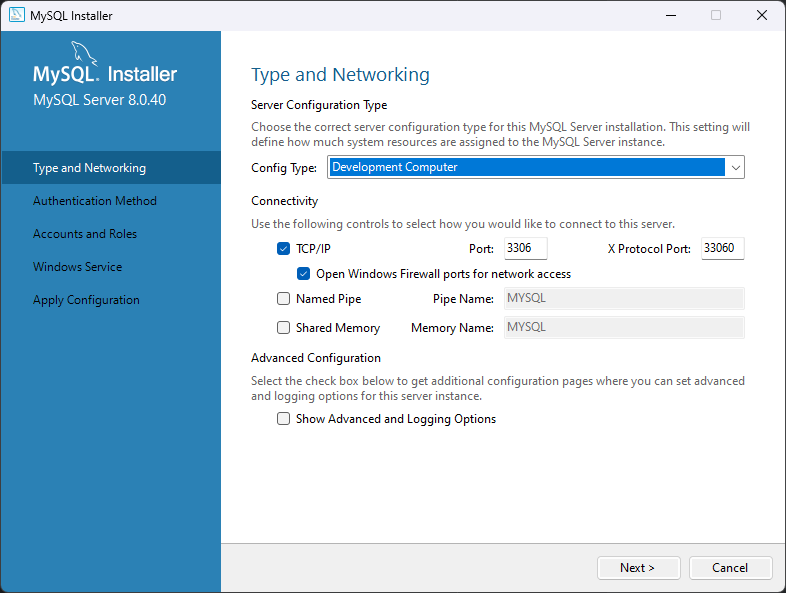
\includegraphics[width=\textwidth]{images/configure.png}
    \caption{配置MySQL}\label{configure}
\end{figure}

然后如图\ref{connect}所示,在PyCharm(Professional Edition)中连接MySQL数据库。

\begin{figure}[!htbp]
    \centering
    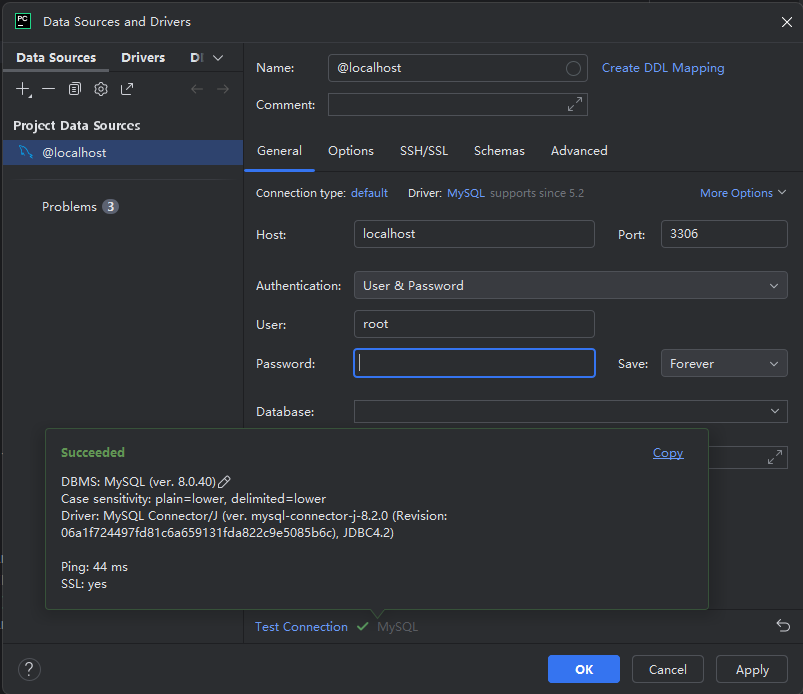
\includegraphics[width=\textwidth]{images/connect.png}
    \caption{连接MySQL}\label{connect}
\end{figure}

接着如图\ref{run}所示,右键点击数据库图标,在菜单中选中“SQL Scripts”,然后点击“Run SQL Script”以运行事先准备好的SQL脚本init\_transaction.sql。

\begin{figure}[!htbp]
    \centering
    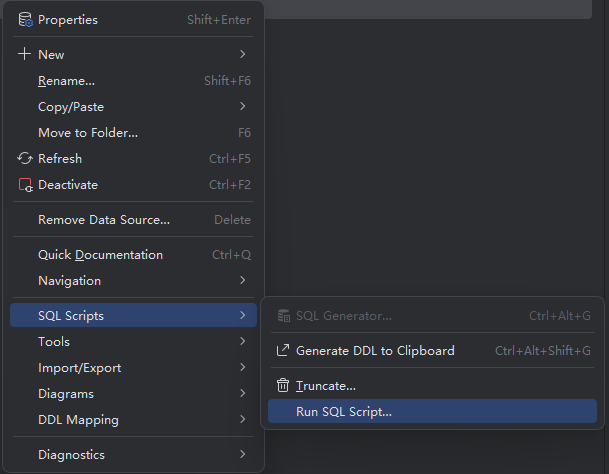
\includegraphics[width=\textwidth]{images/run_script.png}
    \caption{运行SQL脚本文件}\label{run}
\end{figure}

运行后的数据库状态如图\ref{db1}所示。

\begin{figure}[!htbp]
    \centering
    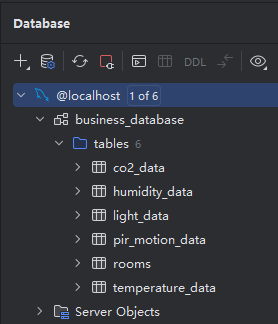
\includegraphics[scale=1]{images/db1.png}
    \caption{运行脚本后的数据库}\label{db1}
\end{figure}


\subsubsection{模拟传感器数据}

创建transaction.ipynb以模拟传感器数据导入业务数据库中的过程。如图\ref{import}所示,传感器数据成功从csv文件中导出。

\begin{figure}[!htbp]
    \centering
    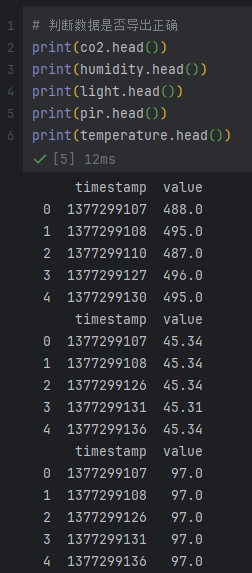
\includegraphics[scale=1]{images/import.png}
    \caption{成功导出传感器数据}\label{import}
\end{figure}


\subsection{数据仓库设计}
我们所设计的数据仓库如图\ref{data}所示。

\begin{figure}[!htbp]
    \centering
    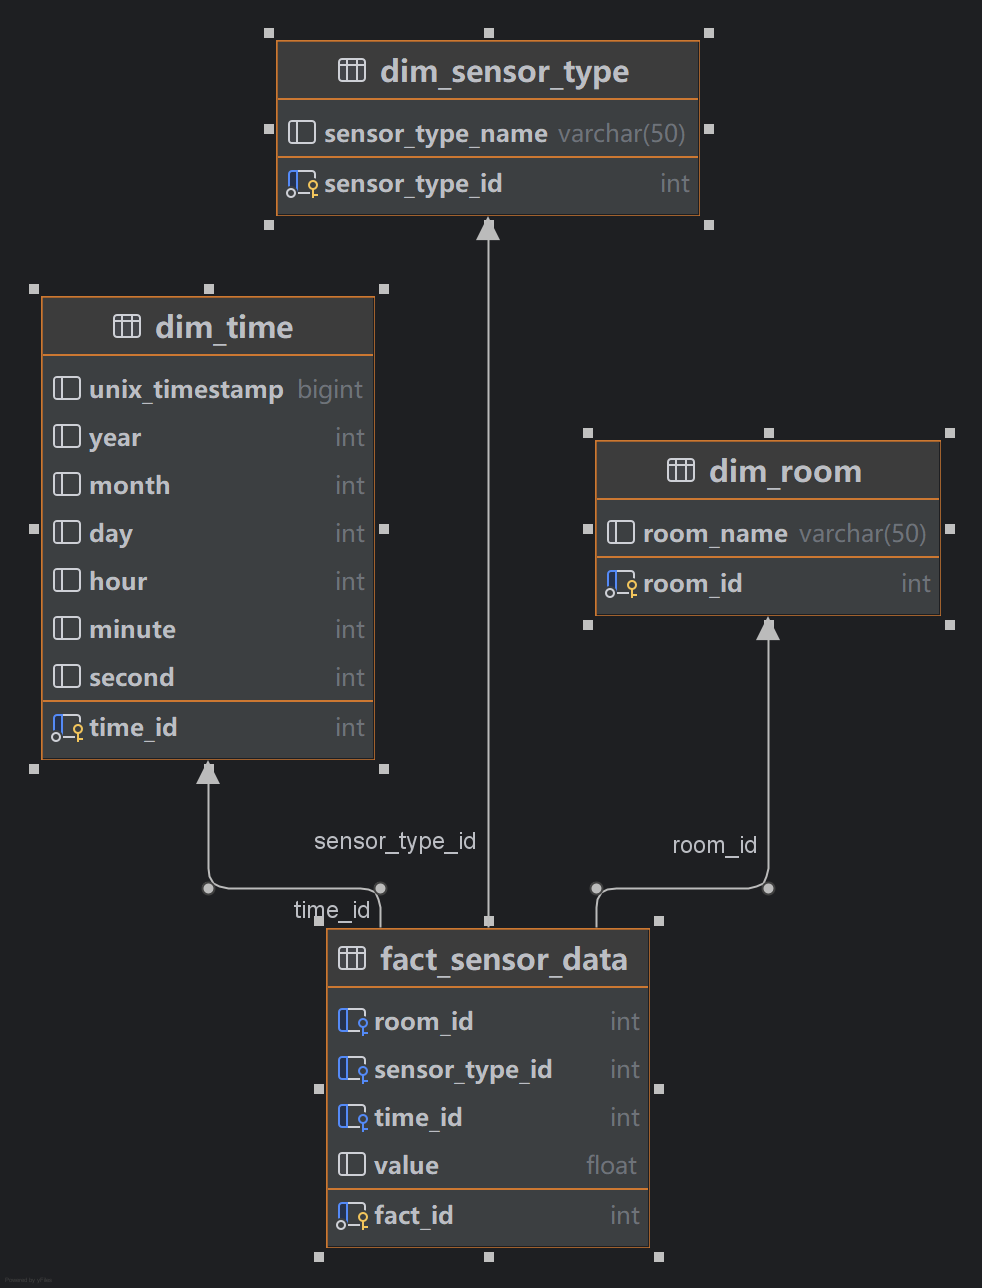
\includegraphics[width=\textwidth]{images/data.png}
    \caption{数据仓库设计}\label{data}
\end{figure}

\subsection{ETL数据插入}
\subsubsection{创建仓库}
和业务数据库一样,我们通过运行事先准备好SQL脚本文件init\_fact.sql来创建数据仓库。运行后的数据库状态如图\ref{db2}所示。

\begin{figure}[!htbp]
    \centering
    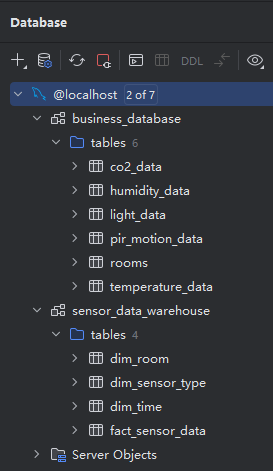
\includegraphics[scale=1]{images/db2.png}
    \caption{运行脚本后的数据库}\label{db2}
\end{figure}

\subsubsection{将数据从业务数据库中加载至数据仓库中}

首先我们从业务数据库中利用SQL语句提取数据,然后利用pandas库生成数据维度数据,最后依次将时间维度数据和事实数据加载至数据仓库中。这一过程通过fact.ipynb文件实现。

\subsection{数据查询}

我们利用query.ipynb文件进行数据查询操作。查询得到的时间维度的温度走势如图\ref{output}所示。